\documentclass[11pt,a4paper,notitlepage,twoside,openright]{report}
\usepackage[utf8]{inputenc}
\usepackage[english]{babel}

\usepackage{color}
\usepackage[table]{xcolor}
\usepackage[export]{adjustbox}
\usepackage{caption}
\usepackage{subcaption}
\usepackage{cite}
\usepackage{amsmath,scalefnt}
\usepackage{amsfonts}
\usepackage{amssymb}
\usepackage{makeidx}
\usepackage{graphicx}
\usepackage{lmodern}
\usepackage{kpfonts}
\usepackage{fancyhdr, blindtext}
\usepackage{float}
\usepackage{multirow}
\usepackage{setspace}

% CHAPTER TITLE FORMATS
\usepackage{titlesec}
\titleformat{\chapter}[display]{\normalfont\huge\bfseries}{\chaptertitlename\ \thechapter}{0pt}{\Huge}   
\titlespacing*{\chapter}{0pt}{10pt}{10pt}
\setcounter{secnumdepth}{3}

% ADDED THESE PACKAGES
\usepackage{soul}   % for highlighting text
\usepackage{bm}     % Bold math
\usepackage{siunitx} % SI units
\usepackage[version=4]{mhchem}
\usepackage{amsthm}
\theoremstyle{definition}   % Include a definition
\newtheorem{definition}{Definition}[section]
\usepackage{booktabs}
\usepackage{gensymb}
\usepackage{algorithm} % include algorithm pseudocode
\usepackage[noend]{algpseudocode}
\usepackage[hidelinks]{hyperref}
\usepackage{appendix}
\usepackage{xfrac}
\usepackage{annotate-equations}
\usepackage{cleveref}

% GEOMETRY
\usepackage[inner=3.5cm,outer=2.5cm,top=2.5cm,bottom=2.5cm]{geometry}

% Nomenclature
\usepackage[intoc]{nomencl} 
\makenomenclature
\renewcommand{\nomname}{List of Symbols}
\newlength{\nomitemorigsep}
\setlength{\nomitemorigsep}{\nomitemsep}
\setlength{\nomitemsep}{0.0cm}
\setlength{\nomlabelwidth}{3cm}
\usepackage{etoolbox}

% DEFINE the GROUPS 
\renewcommand\nomgroup[1]{%
  \item[\Large\bfseries
  \ifstrequal{#1}{P}{Physical constants}{%
  \ifstrequal{#1}{L}{Latin symbols}{%
  \ifstrequal{#1}{G}{Greek Symbols}{%
  \ifstrequal{#1}{C}{Coordinate Systems}{%
  \ifstrequal{#1}{O}{Other Symbols}{%
  \ifstrequal{#1}{S}{Operators, Subscripts and Superscripts}{}}}}}}%
]}
\newcommand{\nomunit}[1]{%
\renewcommand{\nomentryend}{\hspace*{\fill}#1}}

% References
\usepackage[square, numbers, comma, sort&compress]{natbib}
\bibliographystyle{unsrtnat}

% Glossaries
\usepackage[acronym, nonumberlist, nopostdot]{glossaries}
\makeglossaries

% Add custom commands
\newcommand{\versor}[1]{\boldsymbol{\hat{#1}}}
\newcommand{\vect}[1]{\boldsymbol{\mathbf{#1}}}
\newcommand{\mat}[1]{\boldsymbol{\mathbf{#1}}}
\newcommand{\todo}[1]{\textbf{\color{red}[TODO]}: #1}
\newcommand{\gaussian}[2]{\mathcal{N}(#1,\,#2)}

%% ----------------------------------------------------------------
%% ----------------------------------------------------------------
\author{Thomas Barbier}
\begin{document}

%% ----------------------------------------------------------------
% Format Document
\setstretch{1.3} 	
\fancyhead{}  		
\lhead{}  			

\pagestyle{fancy}
\pagenumbering{roman}

%% ----------------------------------------------------------------
% Start creating cover pages and abstracts
\begin{titlepage}
	\centering
	
\includegraphics[width=0.2\textwidth]{Figures/US}
	\par\vspace{1cm}
	
	{\scshape\huge University of Surrey}
		\vspace{1cm}	

	{\scshape\LARGE Surrey Space Centre}\\
	{\scshape Faculty of Engineering and Physical Sciences\\Guildford, Surrey GU2 7XH, U.K.}
       \vspace{1cm}		
	
	{\huge\bfseries Space debris state estimation \\onboard a chaser spacecraft  \par}
	\vspace{1.0cm}
	
	{\Large\itshape Thomas \textsc{Barbier} \par}
	\vspace{1.0cm}
	
	{\scshape\large Submitted for the Degree of \\
		Doctor of Philosophy}
	\vspace{1.0cm}

	Supervisors \\
	Yang \textsc{Gao}\\ 

    \vspace{0.5cm}
    Co-supervisor \\
	Saber \textsc{Fallah}\\ 
	
%    \vspace{0.5cm}
%    External supervisors \\
%	Supervisor \textsc{Name}\\ 
	\vspace{2cm} % 1cm initially
	
	\large March 2023\par

\end{titlepage}
\clearpage


\chapter*{}

\vspace{12cm}

{\Large\textbf{Declaration of Originality}}
\\	

This thesis and the work to which it refers are the results of my own efforts. Any ideas, data, images or text resulting from the work of others (whether published or unpublished) are fully identified as such within the work and attributed to their originator in the text, bibliography or in footnotes. This thesis has not been submitted in whole or in part for any other academic degree or professional qualification. I agree that the University has the right to submit my work to the plagiarism detection service TurnitinUK for originality checks. Whether or not drafts have been so-assessed, the University reserves the right to require an electronic version of the final document (as submitted) for assessment as above.
\\
\\

Signed: ...................................................................................................................... 
\\

Date: ..........................................................................................................................

\clearpage


\chapter*{}

\vspace{6cm}

\begin{center}
    \lq\lq La vie n'a pas de sens, mais vaut la peine d'être vécue, à condition de reconnaître qu'elle n'a pas de sens.\rq\rq \\	
\end{center}
\begin{flushright}
    Albert Camus  
\end{flushright}
\clearpage

\chapter*{Abstract}
\label{cha:Abstract}
\begin{center}
    \normalfont\huge\bfseries Abstract
\end{center}

Add Abstract ...




\addcontentsline{toc}{chapter}{Abstract}
\clearpage

\cleardoublepage
\phantomsection % Required to fix issue with page numbering
\addcontentsline{toc}{chapter}{Acknowledgements}
\chapter*{Acknowledgements}
\label{cha:Acknowledgements}

Add Acknowledgements ...
\lhead{\textit{Acknowledgements}}
\clearpage

% Table of Contents
\lhead{\textit{Contents}} 
\setcounter{tocdepth}{2}
\tableofcontents 
\clearpage

\cleardoublepage
\phantomsection
\addcontentsline{toc}{chapter}{\listfigurename}
\lhead{\textit{List of Figures}}
\listoffigures  % Write out the List of Figures
\clearpage

\cleardoublepage
\phantomsection
\addcontentsline{toc}{chapter}{\listtablename}
\lhead{\textit{List of Tables}}
\listoftables 
\clearpage

\cleardoublepage
\phantomsection
\addcontentsline{toc}{chapter}{List of Acronyms}
\lhead{\textit{List of Acronyms}}
% Acronyms to include
\newacronym{GEO}{GEO}{Geostationary orbit}
\newacronym{RSO}{RSO}{resident space object}
\newacronym{gp}{GP}{Gaussian Process}
\newacronym{gps}{GPs}{Gaussian Processes}
\newacronym{COEs}{COEs}{Classical Orbital Elements}
\newacronym{raan}{RAAN}{Right Ascension of the Ascending Node}
\newacronym{ADR}{ADR}{Active Debris Removal}
\newacronym{SLAM}{SLAM}{Simultaneous Localisation and Mapping}
\newacronym{ACS}{ACS}{Attitude Control Subsystem}
\newacronym{EKF}{EKF}{Extended Kalman Filter}
\newacronym{CAM}{CAM}{Collision Avoidance Manoeuvre}
\newacronym{ESA}{ESA}{European Space Agency}
\newacronym{LEO}{LEO}{Low Earth Orbit}
\newacronym{ECI}{ECI}{Earth Centred Inertial}
\newacronym{LVLH}{LVLH}{Local Vertical Local Horizontal}
\newacronym{ESKF}{ESKF}{Error-State Kalman Filter}
\newacronym{UKF}{UKF}{Unscented Kalman Filter}
\newacronym{Vespa}{Vespa}{Vega Secondary Payload Adapter}
\newacronym{AOCS}{AOCS}{Attitude and Orbit Control Subsystem}
\newacronym{MMX}{MMX}{Martian Moon eXplorer}
\newacronym{MIRs}{MIRs}{Moments of Inertia Ratios}
\newacronym{TRL}{TRL}{Technology Readiness Level}
\newacronym{VBN}{VBN}{Vision-Based Navigation}
\newacronym{OOS}{OOS}{On-Orbit Servicing}
\newacronym{ODE}{ODE}{Ordinary Differential Equation}
\newacronym{FFT}{FFT}{Fast Fourier Transform}
\newacronym{CoM}{CoM}{Center of Masss}
\newacronym{YA}{YA}{Yamana-Ankersen}
\newacronym{CW}{CW}{Clohessy-Wiltshire}
\newacronym{ssa}{SSA}{space situational awareness}
\newacronym{rso}{RSO}{resident space object}
\newacronym{adr}{ADR}{active debris removal}
\newacronym{oos}{OOS}{on-orbit servicing}
\newacronym{od}{OD}{orbit determination}
\newacronym{sd}{SD}{space debris}
\newacronym{pdf}{PDF}{probability density function}
\newacronym{neo}{NEO}{near-Earth orbits}
\newacronym{us}{US}{United States}
\newacronym{eu}{EU}{European Union}
\newacronym{ssn}{SSN}{space surveillance network}
\newacronym{sst}{SST}{space surveillance and tracking}
\newacronym{fov}{FOV}{field of view}
\newacronym{esa}{ESA}{European Space Acency}
\newacronym{nasa}{NASA}{National Aeronautics and Space Administration}
\newacronym{leo}{LEO}{Low-Earth orbit}
\newacronym{geo}{GEO}{geostationary Earth orbit}
\newacronym{meo}{MEO}{medium-Earth orbit}
\newacronym{heo}{HEO}{highly-elliptical orbit}
\newacronym{tle}{TLE}{two-line element}
\newacronym{eci}{ECI}{Earth-centered inertial}
\newacronym{ode}{ODE}{ordinary differential equation}
\newacronym{grv}{GRV}{Gaussian random variable}
\newacronym{gto}{GTO}{geostationary transfer orbit}
\newacronym{dof}{DoF}{Degrees of Freedom}
\newacronym{eom}{EoM}{equations of eotion}
\newacronym{ukf}{UKF}{unscented Kalman filter}
\newacronym{ekf}{EKF}{extended Kalman filter}
\newacronym{kep}{KEP}{Keplerian classical Elements}
\newacronym{cc}{CC}{cartesian Coordinates}
\newacronym{pf}{PF}{particle filter}
\newacronym{ls}{LS}{least square}
\newacronym{nls}{NLS}{non-linear least square}
\newacronym{iss}{ISS}{international space station}
\newacronym{cots}{COTS}{component off the shelf}
\newacronym{roi}{ROI}{return of investment}
\newacronym{cam}{CAM}{collision avoidance manoeuvre}
\newacronym{vbn}{VBN}{vision-based navigation}
\newacronym{see}{SEE}{single-event effect}
\newacronym{mli}{MLI}{multi-layer insulation}
\newacronym{slam}{SLAM}{simultaneous localisation and mapping}
\newacronym{eol}{EOL}{End Of Life}
\newacronym{oe}{OE}{Opto-Electronic}
\newacronym{iadc}{IADC}{Inter-Agency Space Debris Coordination}
\newacronym{asat}{ASAT}{Anti-Satellite}
\newacronym{cad}{CAD}{Computer-Aided Design}
\newacronym{atv}{ATV}{Automated Transfer Vehicle}
\newacronym{imu}{IMU}{Inertial Measurement Unit}
\newacronym{led}{LED}{Light-Emitting Diode}
\newacronym{lidar}{LiDAR}{Light Detection And Ranging}
\newacronym{sift}{SIFT}{scale-invariant feature transform}
\newacronym{surf}{SURF}{speeded-up robust feature}
\newacronym{brief}{BRIEF}{binary robust independent elementary features}
\newacronym{fast}{FAST}{features from accelerated segment test}
\newacronym{orb}{ORB}{oriented FAST and rotated BRIEF}
\newacronym{freak}{FREAK}{fast retina keypoint}
\newacronym{ransac}{RANSAC}{random sample consensus}
\newacronym{cnes}{CNES}{Centre National d'Études Spatiales}
\newacronym{sfm}{SfM}{structure from motion}
\newacronym{ba}{BA}{bundle adjustment}
\newacronym{wba}{WBA}{windowed bundle adjustment}
\newacronym{vo}{VO}{visual odometry}
\newacronym{cnn}{CNN}{convolutionnal neural network}
\newacronym{cw}{CW}{Clohessy - Wiltshire}
\newacronym{ya}{YA}{Yamanaka - Ankersen}
\newacronym{aocs}{AOCS}{attitude and orbit control subsystem}
\newacronym{lm}{LM}{Levenberg-Marquardt}
\newacronym{gn}{GN}{Gauss-Newton}
\newacronym{gd}{GD}{gradient-descent}
\newacronym{lvlh}{LVLH}{local vertical local horizontal}
\newacronym{cog}{CoG}{center of gravity}
\newacronym{dl}{DL}{Dog-Leg}
\newacronym{acs}{ACS}{attitude control system}
\newacronym{api}{API}{Application Programming Interface}
\newacronym{lk}{LK}{Lucas-Kanade}
\newacronym{klt}{KLT}{Kanade-Lucas-Tomasi}
\newacronym{pw}{PW}{Pulse-Wave}
\newacronym{cw}{CW}{Continuous-Wave}
\newacronym{tof}{TOF}{Time of Flight}
% --------------------------------------------------------
% Set Style
\setglossarystyle{long}
\renewcommand{\arraystretch}{1.2}
\renewcommand{\glsnamefont}[1]{\textbf{#1}}
\setlength\LTleft{2pt}
\setlength\LTright{0pt}
\setlength\glsdescwidth{1.5\hsize}
% --------------------------------------------------------

\printglossary[type=\acronymtype,title={List of Acronyms},style=long,nogroupskip=true]
\clearpage

\cleardoublepage
\phantomsection
\lhead{\textit{List of Symbols}}
%% This code DEFINES the symbols
\renewcommand{\arraystretch}{1.0}
% Physical Constants
\nomenclature[P]{\(G\)}{gravitational constant\nomunit{\SI[group-digits=false]{6.67430e-11}{\meter\cubed\per\kilogram\per\second\squared}}}
\nomenclature[P]{\(g_0\)}{standard gravitational field strength\nomunit{\SI[group-digits=false]{9.80665}{\meter\per\second\squared}}}

% Different group
\nomenclature[G]{\(\mu\)}{mass parameter}
\printnomenclature
\clearpage

%% ----------------------------------------------------------------
%% ----------------------------------------------------------------
% Actual content for the document
\pagestyle{fancy}
\pagenumbering{arabic}

\lhead{\textit{Introduction}}
\chapter{Introduction}
\label{cha:intro}

%------------------------------------------------------------------------------
%------------------------------------------------------------------------------
\section{Space Debris}
\label{intro:space_debris}
% Introduction of the space debris problem
Since the launch of the first artificial satellite, Sputnik 1, by the USSR in 1957, human activities in space never ceased to grow. With only 3 satellites launched to \Gls{geo} in 1970, 2015 alone was the year of 35 new satellites into the same \gls{geo}. When it comes to the \Gls{leo}, those numbers are even more striking as we ramp up from 100 satellites launches in 1970 to over 400 in 2018. While the number of satellites put on that orbit remained quite steady with a mean of roughly 70 satellites per year, 2010 was the beginning of the so-called \emph{New-Space} movement where space activities gradually shifted from a government and big companies niche towards being more affordable for smallest companies and universities. \gls{leo} missions took advantage of the introduction of \Gls{cots} and new launches services such as \emph{SpaceX}, \emph{Rocket Lab} or directly from the \Gls{iss} which, once combined, drastically decrease the building and launching cost of a satellite. \gls{geo} on its side remains the preserve of the big historical constructors and operators because of its very particular use and constraints which makes it very costly. \Gls{roi} of such missions (mainly telecommunications) makes it very attractive, explaining the growing number of launched payload each year.


%   Three ways of dealing with it: Keeping track for manipulations, EOL, Active debris removal
Space Debris problem can be tackled in three ways:
\begin{itemize}
    \item \textbf{Cataloguing and tracking}: through a thorough observation via radars and telescope a catalogue of known debris is created with their estimated orbital parameters. Their orbits can then be propagated and when a collision risk is detected, then a manoeuvre can be performed to maintain the spacecraft's integrity and mission.
    \item \textbf{End of life guidelines}: space agencies around the world integrated as a guideline the re-entry of \gls{leo} satellites no later than 25 years after decommission. When arriving at its end of life, the satellite must then perform some manoeuvre and actions (such as passivation) to enable a safe, passive re-entry in the allowed timescale. \emph{Surrey Space Centre} pioneered the use of a drag-sail to considerably reduce the reentry time-frame of their technology demonstrator mission \emph{Remove Debris} without using any propulsion device \citep{forshaw_removedebris:_2016}. \gls{geo} requires a manoeuvre towards a graveyard orbit 300km higher than nominal orbit. However, those guidelines have a cost for spacecraft manufacturers and operators, adding weight, fuel or component to the spacecraft, which makes them rarely applied in the commercial world. Since 2008, the French Space Operations Act enforces the application of those end of life guidelines for every satellite that is partly or entirely manufactured, operated or launched by a French company.
    \item \textbf{\gls{adr}}: mitigating debris creation through the extensive use and application will still leave room for risks from actual debris. Furthermore, with the kilo-constellation projects such as \emph{SpaceX} or \emph{One Web}, \gls{adr} missions will soon become necessary to ensure sustainable use of space and keeping the collision risk as low as possible. \emph{Remove Debris} mission from \emph{Surrey Space Centre} investigated and tested the use a net and a harpoon to such an end.
\end{itemize}


\gls{adr} mission can be decomposed in several steps. First, specific debris from the catalogue has to be chosen to get rid off. Knowledge of this debris can be various depending on its nature (fully known decommissioned satellite or piece of a rocket body explosion). As stated above, we will make here no assumption on prior knowledge of the debris except on its estimated orbital elements from the space debris catalogue (thus enabling propagation of its orbital state and, in fine, a rendezvous manoeuvre to its vicinity). Then the observation phase takes place where the chaser manoeuvre actively or passively (thanks to relative orbital mechanics) around the target (debris) to take measurements, followed by the active capture phase. Finally, the chaser moves the target either to re-entry or graveyard orbit. 
%A conceptual graph of mission phases can be found in fig. \ref{fig:adr_phases}. 
%\todo{Make a graph of the different phases}

Proximity operations of phases 2 and 3 are highly risked as any substantial error in the estimation or control could lead to a collision between the chaser and the target leading to a potential loss of the mission upon creating new debris. The scientific community tried to alleviate this problem by introducing \emph{relative navigation} and more especially \gls{vbn}. In case of a grasping or docking scenario of the chaser to the target, furthermore computations are required to estimate the shape and kinematic properties of the latter to decide \emph{where} and \emph{how} the chaser will dock/grasp.

% The state of computers in space
Those estimation and control problems can find an echo into the terrestrial robotic and aeronautical community where they already are partially or fully solved. However, space remains an outer and challenging domain with its own and very specific constraints. Above all is the harsh environment which makes ground computers often irrelevant for space applications. Radiation levels involved makes radiation-hardened hardware required to withstand \gls{see}. This can be done by additional shielding, robust computing design (monitoring with separate code, vote scheme, re-computation), robust hardware architecture etc. All those constraints lead to an immense gap between computing power available on-ground compared to the one available on-board of a spacecraft. The latest development in LEON processors, Europe's space computers flagship, is the quad-core GR740 clocked at roughly 250MHz \citep{staff_space-grade_2019}. The harsh environment also imposes many poor measurement conditions such as harsh lighting conditions where the dynamic range of a camera can't keep up with sun illumination in the background, or simply having no illumination during the night phase. LiDAR measurements as well can be error-prone due to the reflective nature of the \gls{mli} of other materials used on the object.
% The risk in space that has to be very small.
%   Decrease the risk of space missions in general
%   Have an ADR mission that is as less risky as possible

%------------------------------------------------------------------------------
%------------------------------------------------------------------------------
\section{Autonomous navigation around and unknown target}
\label{intro:autonomous_navigation}

%------------------------------------------------------------------------------
%------------------------------------------------------------------------------
\section{Research aims and Objectives}
\label{intro:research_aims}

%------------------------------------------------------------------------------
%------------------------------------------------------------------------------
\section{Conferences, Workshops and Publications}
\label{intro:papers}

%------------------------------------------------------------------------------
%------------------------------------------------------------------------------
\section{Outline of the thesis}
\label{intro:outline}


\clearpage

\lhead{\textit{Chapter2}}
\chapter{Background}\label{cha:Chapter2}
This chapter discusses the relevant background theory and state-of-the-art in the literature. First, fundamental concepts around space dynamics are considered in \cref{C2:space_dynamics} with concepts such as relative motion and tumbling dynamics. Onboard sensing capabilities are then discussed in \cref{C2:sensing} with a flown hardware on-board previous mission followed by an emphasis on image processing. \Cref{C2:filters} introduces Kalman filtering and its variants of interest for the present work. Finally, \gls{gps} are introduced in \cref{C2:gaussian_processes} with their mathematical description and we explore the choice of their covariance function. In order to deepen one or more of these topics, the reader is invited to read the book by Schaub and Junkins \cite{schaub_analytical_2003} for Space mechanics, Szeliski \cite{szeliski_computer_2011} and Hartley and Zisserman \cite{hartley_multiple_2003} for cameras and image processing, Simon \cite{simon_optimal_2006} on Kalman filtering, and finally Murphy \cite{murphy_machine_2012} on Machine Learning.

%------------------------------------------------------------------------------
%------------------------------------------------------------------------------
\section{Preliminaries}\label{C2:notation_ref_frames}
In this work, the problem of capturing one spatial object by another is addressed. As such, we will refer to the at the satellite operating the estimation on which we embark the proposed algorithm as \emph{the chaser}, and the space debris being estimated as \emph{the target}. The following subsection detail the various frames used in this document as well as outlining the notation used to express different quantities in the specified frames.

\subsection{Reference frames}
Throughout this work, the following frames are used:
\begin{itemize}
	\setlength\itemsep{0em}
	\item $\{N\}$: Inertial frame, defined as \gls{ECI} frame.
	\item $\{L\}$: \gls{LVLH} frame, defined with $z$ pointing at Earth, $y$ in the opposite direction of angular momentum and $x$ as the cross-product of the first two to make a right-handed coordinate frame (in the case of perfectly circular orbit, $x$ matches the direction of the velocity vector of the spacecraft).
	\item $\{C\}$: The chaser frame. Sensor values are expressed in this frame to lighten the notation. On a real spacecraft, the transformation between sensors frame and chaser's main frame is assumed to be fully known (by design and calibration). Data can therefore be easily transformed from one frame to another.
	\item $\{B\}$: The space debris, also referred to as \emph{target}, main body frame. Centred at the target centre of mass, its axis corresponds to its main axis of inertias.
	\item $\{M\}$: A fixed target frame. The rotation $[MB] = cst. \; \forall t$
\end{itemize}

\subsection{Notation}
Quantities are expressed using the following formalism: $^{L}\boldsymbol{r}_{CB}$ is the vector denoting the position of $\{C\}$ (Chaser) with regard to $\{B\}$ (estimated Body, here the target) expressed in $\{L\}$ (\gls{LVLH}) frame. When a quantity is expressed in or regarding the inertial frame, we might omit the subscript $N$ for conciseness (ex: $\boldsymbol{\omega}_B = \: ^{N}\boldsymbol{\omega}_{BN}$). Rotations can be expressed either as a rotation matrix or a quaternion. In the first case, it is expressed using the two letters of the frames of the transformation. For example, given a point $p$, we have: $^Bp = \text{[BN]} \: ^Np$. In case of a representation with a quaternion, the same rotation is written as $\boldsymbol{q}_{BN}$.


%------------------------------------------------------------------------------
%------------------------------------------------------------------------------
\section{Space dynamics}\label{C2:space_dynamics}

%------------------------------------------------------------------------------
\subsection{Orbital dynamics}

\subsubsection{Orbital motion}
In case of the \emph{Two Body} problem, a first yet very useful approximation of gravity is expressed with the Newtonian equation of gravitation. For two point masses $m_1$ and $m_2$, the acting force of one body to the other can be expressed as:
\begin{equation}
	\vect{F}=-G \frac{m_1 m_2}{r^3} \vect{r}
\end{equation}
with $G$ the universal gravitational constant and $\vect{r}$ the vector from one point-mass to the other. In the case of satellites orbiting the Earth, the mass of the planet is much greater than the mass of the satellite, so the latter can be neglected. Using $\vect{F} = m_{sat}\vect{a} = m_{sat}\ddot{\vect{r}}$ and $\mu = G m_{earth}$, we can rewrite the above equation and express the acceleration of a satellite in subject to earth's gravity as:
\begin{equation}
	\ddot{\vect{r}} = -\mu \frac{\vect{r}}{\left\| \vect{r} \right\|^3}
\end{equation}
The above equation can be integrated to reconstruct the motion of the spacecraft around the Earth under the assumption of no external perturbations, also known as Keplerian motion.

Instead of using the state $\vect{x} = \left[\vect{r},\; \vect{\dot{r}}\right]$, the orbit around a central body is usually described using the \gls{COEs} which comprises 6 elements:
\begin{itemize}
	\item $a$: semi-major axis
	\item $e$: eccentricity
	\item $i$: inclination
	\item $\Omega$: \gls{raan}
	\item $\omega$: argument of the periapsis
	\item $\nu$: true anomaly
\end{itemize}

\begin{figure}
	\centering
	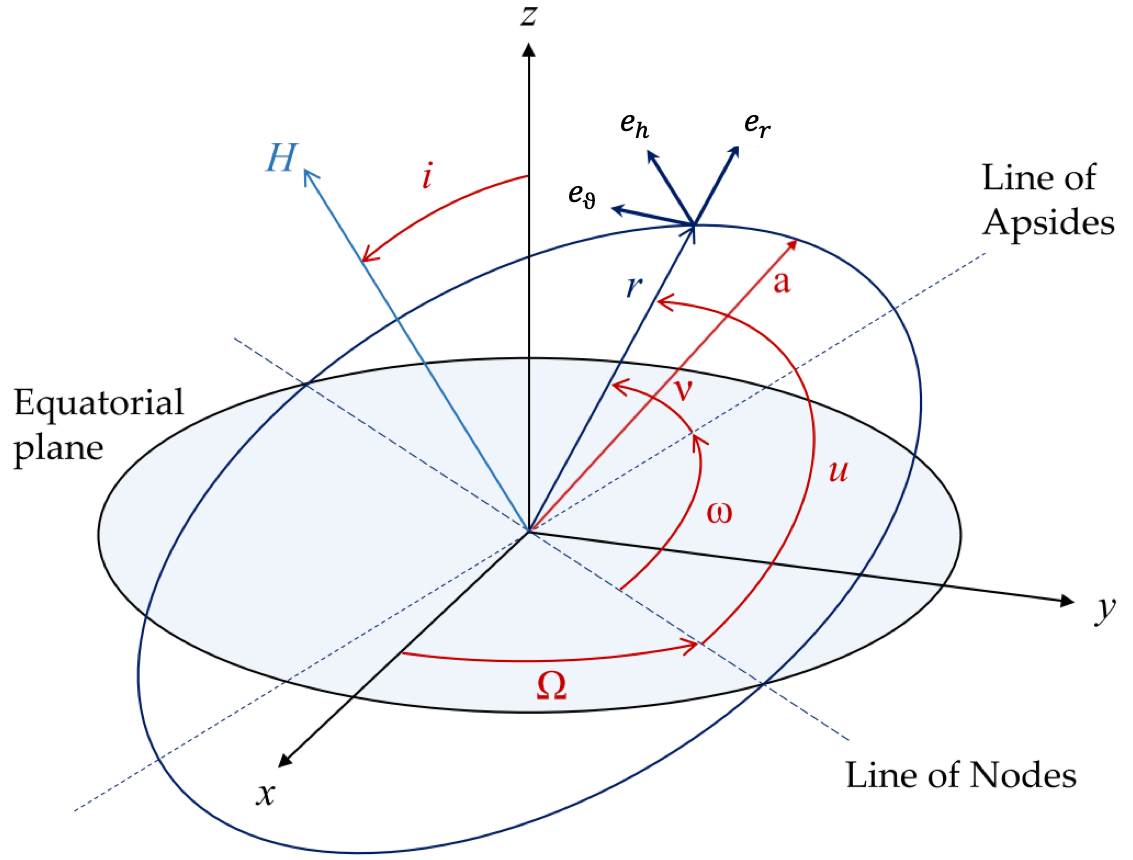
\includegraphics[width=0.8\textwidth]{Figures/orbital_ements}
	\caption{Diagram of the classical orbital elements}
	\label{fig:orbital_elements}
\end{figure}

A representation of the above parameters is presented on \cref{fig:orbital_elements}. For an elliptic orbit, the transition \gls{COEs} to Cartesian coordinates can be performed with the following computation \cite{schaub_analytical_2003}:

\begin{equation}
	\begin{bmatrix}
		\vect{r} \\
		\vect{\dot{r}}
	\end{bmatrix} = 
	\begin{bmatrix}
		r \left( \cos{\left({{\Omega}}\right)} \cos{\left({{\omega} + {\nu}}\right)} - \sin{\left({{\Omega}}\right)} \sin{\left({{\omega} + {\nu}}\right)} \cos{\left({i}\right)} \right)\\ 
		r \left( \cos{\left({{\Omega}}\right)} \cos{\left({{\omega} + {\nu}}\right)} - \sin{\left({{\Omega}}\right)} \sin{\left({{\omega} + {\nu}}\right)} \cos{\left({i}\right)} \right)\\
		r \sin{\left({{\omega} + {\nu}}\right)} \sin{\left({i}\right)}\\ 
		\frac{-{\mu}}{h} \left( \cos{\left({{\Omega}}\right)} \left( \sin{\left({{\omega} + {\nu}}\right)} + e \sin{\left({{\omega}}\right)} \right) + \sin{\left({{\Omega}}\right)} \left( \cos{\left({{\omega} + {\nu}}\right)} + e \cos{\left({{\omega}}\right)} \right) \cos{\left({i}\right)} \right)\\ 
		\frac{-{\mu}}{h} \left( \sin{\left({{\Omega}}\right)} \left( \sin{\left({{\omega} + {\nu}}\right)} + e \sin{\left({{\omega}}\right)} \right) - \cos{\left({{\Omega}}\right)} \left( \cos{\left({{\omega} + {\nu}}\right)} + e \cos{\left({{\omega}}\right)} \right) \cos{\left({i}\right)} \right)\\
		\frac{-{\mu}}{h} -\left( \cos{\left({{\omega} + {\nu}}\right)} + e \cos{\left({{\omega}}\right)} \right) \sin{\left({i}\right)}
	\end{bmatrix}
\end{equation}
with $p$ the semi-latus rectum, $r$ the orbit radius and $h$ the orbital angular magnitude:
\begin{align}
	p &= a \left( {1.0} - e^2 \right) \\ 
	r &= \frac{p}{{1.0} + e \cos{\left({{\nu}}\right)}} \\ 
	h &= \sqrt{{\mu} p}
\end{align}

Equally, Cartesian states can be converted to \gls{COEs} in a similar, straightforward fashion:
\begin{equation}
	\begin{bmatrix}
		e \\ a \\ i\\ \Omega \\ \omega \\ \nu
	\end{bmatrix} = \begin{bmatrix}
			\left| \vect{e} \right| \\
			\frac{1}{\frac{2}{\left\| \vect{r} \right\|} - \frac{\vect{\dot{r}} \times \vect{r}}{\mu}} \\
			\cos^{-1}\left( C_{33}\right) \\
			\tan^{-1}\left(\frac{C_{31}}{C_{32}}\right) \\
			\tan^{-1}\left(\frac{C_{13}}{C_{23}}\right) \\
			\tan^{-1}\left(\frac{( \vect{\imath}_e \times \vect{\imath}_r) \cdot \vect{\imath}_h}{\vect{\imath}_e \cdot \vect{\imath}_r}\right)
		\end{bmatrix}
\end{equation}
with the unit vectors $\vect{i}_e$, $\vect{i}_p$ and $\vect{i}_h$ defined as:
\begin{align}
	\boldsymbol{\imath}_e &=\boldsymbol{e} / e=C_{11} \boldsymbol{\imath}_x+C_{12} \boldsymbol{\imath}_y+C_{13} \boldsymbol{\imath}_z \\
	\boldsymbol{\imath}_p &=\boldsymbol{\imath}_h \times \boldsymbol{\imath}_e=C_{21} \boldsymbol{\imath}_x+C_{22} \boldsymbol{\imath}_y+C_{23} \boldsymbol{\imath}_z \\
	\boldsymbol{\imath}_h &=\boldsymbol{h} / h=C_{31} \boldsymbol{\imath}_x+C_{32} \boldsymbol{\imath}_y+C_{33} \boldsymbol{\imath}_z
\end{align} and:
\begin{align}
	\vect{e} &= \frac{\vect{\dot{r}} \times \vect{h}}{\mu} - \frac{\vect{r}}{\left\| \vect{r} \right\|} \\
	\vect{h} &= \vect{r} \times \vect{\dot{r}}
\end{align}

While \gls{COEs} are preferred to describe the orbit of a given satellite, close-proximity operations, involving manoeuvres in the vicinity of a target, are often expressed in Cartesian coordinates for ease of use \cite{labourdette_trajectoires_2015}.


\subsubsection{Relative motion}
In the case of a chaser-target configuration, also known as \emph{formation flying}, the relative motion between the two objects is of importance for the mission. In the case of two Keplerian orbit, the target Cartesian state $^{L}\vect{x}_B = \left[^{L}\vect{r}_B \: ^{L}\vect{\dot{r}}_B \right]$ expressed in the chaser-centred \gls{LVLH} frame is given through the integration of the following \gls{ODE} using the chaser's\gls{COEs}:

\begin{equation} \label{eq:eq_diff_rel_motion}
	\left[ \begin{array} { c } { \ddot { x } } \\ { \ddot { y } } \\ { \ddot { z } } \end{array} \right] = \left[ \begin{array} { c } { - k \theta ^ { \frac { 3 } { 2 } } x + 2 \theta \dot { z } + \dot { \theta } z + \theta ^ { 2 } x } \\ { - k \theta ^ { \frac { 3 } { 2 } } y } \\ { 2 k \theta ^ { \frac { 3 } { 2 } } z - 2 \theta \dot { x } - \dot { \theta } x + \theta ^ { 2 } z } \end{array} \right]
\end{equation}
with:
\begin{equation}
	n = \sqrt{\frac{\nu}{a^3}}, \quad \theta = \dot{\nu} = \frac{h}{r^2} = n\frac{(1+e\cos{\nu})^2}{(1-e^2)^\frac{3}{2}}, \quad  \dot{\theta} = \ddot{\nu} = n^2\frac{2e\sin{\nu}\:(1+e\cos\nu)^3}{(1-e^2)^3}
\end{equation}

A commonly used analytical solution for circular orbits is the \gls{CW} model \cite{schaub_analytical_2003}. In the case of elliptic, non-circular orbits, however, this solution doesn't generalize. The \gls{YA} model \cite{yamanaka_new_2002} is a proposed solution for all elliptic eccentricities $e$.

Their approach relies on a variable change where they no longer rely on time derivatives but express the equations with the true anomaly, and then do the following variable change:
\begin{equation} \label{eq:ya_variable_change}
	\begin{bmatrix}
		\tilde{x}\\ 
		\tilde{y}\\ 
		\tilde{z}
	\end{bmatrix} = \rho \, \begin{bmatrix}
		x\\ 
		y\\ 
		z
	\end{bmatrix}, \quad \rho = 1+e\cos\nu
\end{equation}{}
which, once plugged into \cref{eq:eq_diff_rel_motion} gives the following system:
\begin{equation} \label{eq:ya_diff_eq_nu}
	\begin{array} { c } { \tilde { x } ^ { \prime \prime } - 2 \tilde { y } ^ { \prime } - \frac { 3 } { \rho } \tilde { x } = 0 } \\ { \tilde { y } ^ { \prime \prime } + 2 \tilde { x } ^ { \prime } = 0 } \\ { \tilde { z } ^ { \prime \prime } + \tilde { z } = 0 } \end{array} \text{where } \tilde{x} = \frac{dx}{d\nu}
\end{equation}{}

\Cref{eq:eq_diff_rel_motion} are also known as \emph{Lawden} \citep{lawden_optimal_1963} or \emph{Tschauner-Hempel} \citep{tschauner_rendezvous_1965} equations. They show a couple motion in the orbital plane (XZ) and an uncoupled sinusoidal motion out-of-plane (Y) which accepts a solution with the form of an harmonic oscillator. From there, the authors can develop their computations leading to the following state-transition matrices in \gls{LVLH} frame attached to the target:

\begin{itemize}
	\item Out-of-plan motion (Y):
	\begin{equation} \label{eq:ya_y}
		\left[ \begin{array} { c } { y ( t ) } \\ { \dot { y } ( t ) } \end{array} \right] = \Psi _ { v } ^ { - 1 } \left[ \begin{array} { c c } { \cos \left( v - v _ { 0 } \right) } & { \sin \left( v - v _ { 0 } \right) } \\ { - \sin \left( v - v _ { 0 } \right) } & { \cos \left( v - v _ { 0 } \right) } \end{array} \right] \Psi _ { v _ { 0 } } \left[ \begin{array} { c } { y \left( t _ { 0 } \right) } \\ { \dot { y } \left( t _ { 0 } \right) } \end{array} \right]
	\end{equation}{}
	with matrices $\Psi _ { v _ { 0 } }$ and $\Psi _ { v } ^ { - 1 }$ the transition matrix from $\tilde{x}$ to $x$ and vice-versa, defined as:
	\begin{equation}\label{eq:ya_matric}
		\Psi _ { v _ { 0 } } = \left[ \begin{array} { c c } { \rho _ { v _ { 0 } } } & { 0 } \\ { - e \sin v _ { 0 } } & { \frac { 1 } { k ^ { 2 } \rho _ { v _ { 0 } } } } \end{array} \right]
		\text{ and }
		\Psi _ { v } ^ { - 1 } = \left[ \begin{array} { c c } { \frac { 1 } { \rho _ { v } } } & { 0 } \\ { k ^ { 2 } e \sin v } & { k ^ { 2 } \rho _ { v } } \end{array} \right]
	\end{equation}{}
	
	\item In-plane motion (XZ):
	\begin{equation}\label{eq:ya_xz}
		\left[ \begin{array} { l } { x ( t ) } \\ { z ( t ) } \\ { \dot { x } ( t ) } \\ { \dot { z } ( t ) } \end{array} \right] = \Psi _ { v } ^ { - 1 } \left[ \Phi _ { v } \Phi _ { v _ { 0 } } ^ { - 1 } \right]  \Psi _ { v _ { 0 } } \left[ \begin{array} { c } { x \left( t _ { 0 } \right) } \\ { z \left( t _ { 0 } \right) } \\ { \dot { x } \left( t _ { 0 } \right) } \\ { \dot { z } \left( t _ { 0 } \right) } \end{array} \right]
	\end{equation}{}
	with matrices $\Phi _ { v }$ and $\Phi _ { v _ { 0 } } ^ { - 1 }$ defined as follow:
	\begin{equation}
		\Phi _ { v _ { 0 } } ^ { - 1 } = \frac{1}{1-e^2}
		\left[ \begin{array} { c c c c } { 1 - e ^ { 2 } } & { 3 e s \left( \frac { 1 } { \rho } + \frac { 1 } { \rho ^ { 2 } } \right)  } & { - e s \left( 1 + \frac { 1 } { \rho } \right) } & { - e c + 2 } \\ { 0 } & { - 3 s \left( \frac { 1 } { \rho } + \frac { e ^ { 2 } } { \rho ^ { 2 } } \right) } & { s \left( 1 + \frac { 1 } { \rho } \right) } & { c - 2 e } \\ { 0 } & { - 3 \left( \frac { c } { \rho } + e \right) } & { c \left( 1 + \frac { 1 } { \rho } \right) + e } & { - s } \\ { 0 } & { 3 \rho + e ^ { 2 } - 1 } & { - \rho ^ { 2 } } & { e s } \end{array} \right] _ { v _ { 0 } }
	\end{equation}{}
	
	\begin{equation}
		\Phi _ { v } = \left[ \begin{array} { c c c c } { 1 } & { - c \left( 1 + \frac { 1 } { \rho } \right) } & { s \left( 1 + \frac { 1 } { \rho } \right) } & { 3 \rho ^ { 2 } J } \\ { 0 } & { s } & { c } & { 2 - 3 e s f } \\ { 0 } & { 2 s } & { 2 c - e } & { 3 ( 1 - 2 e s ) } \\ { 0 } & { s ^ { \prime } } & { c ^ { \prime } } & { - 3 e \left( s ^ { \prime }J + \frac { s } { \rho ^ { 2 } } \right) } \end{array} \right]_v
	\end{equation}{}
	
	and
	\begin{multline}
		J = k^2(t-t_0), \quad k^2 = \frac{\sqrt{\mu}}{p^{^3/_2}}, p=a(1-e^2), \quad \rho = 1+e\cos\nu, \\ 
		s = \rho\sin\alpha, \quad c=\rho\cos\alpha, \quad s^{\prime} = \cos\alpha + e\cos2\alpha, \\
		c ^ { \prime } = -\sin\alpha-e\sin2\alpha, \quad \alpha = \nu \textrm{ or }\nu_0
	\end{multline}{}
	Again, matrices  $\Psi _ { v _ { 0 } }$ and $\Psi _ { v } ^ { - 1 }$ the transition matrix from $\tilde{x}$ to $x$:
	
	\begin{equation}
		\Psi _ { v _ { 0 } } = \left[ \begin{array} { c c c c } { \rho } & { 0 } & { 0 } & { 0 } \\ { 0 } & { \rho } & { 0 } & { 0 } \\ { - e \sin v _ { 0 } } & { 0 } & { \frac { 1 } { k ^ { 2 } \rho } } & { 0 } \\ { 0 } & { - e \sin v _ { 0 } } & { 0 } & { \frac { 1 } { k ^ { 2 } \rho } } \end{array} \right]_ { v_0 }
	\end{equation}{}
	\begin{equation}
		\Psi _ { v } ^{- 1} = \left[ \begin{array} { c c c c } { \frac { 1 } { \rho } } & { 0 } & { 0 } & { 0 } \\ { 0 } & { \frac { 1 } { \rho } } & { 0 } & { 0 } \\ { k ^ { 2 } e \sin v } & { 0 } & { k ^ { 2 } \rho } & { 0 } \\ { 0 } & { k ^ { 2 } e \sin v } & { 0 } & { k ^ { 2 } \rho } \end{array} \right] _ { v }
	\end{equation}{}
\end{itemize}{}

The construction of matrices $\Phi$ ans $\Psi$ requires the knowledge of true anomaly $\nu$ at time $t$. In the general case it uses the iterative resolution of Kepler's equations $M = E + e\sin E$ with $M = M_0 + n\Delta t$ the mean anomaly, $E$ the eccentric anomaly. True anomaly can the then recovered with the relation: $\tan\frac{\nu}{2} = \sqrt{\frac{1+e}{1-e}}\tan\frac{E}{2}$.

A closed-form solutions to the relative motion \gls{ODE} such as the \gls{CW} and \gls{YA} comes in very handy when it is necessary to calculate these quantities on board. Indeed, as the computing power of the computers embedded in satellites is relatively limited, the possibility of propagating the relative states using linear algebra rather than an integrator is of great value.


%------------------------------------------------------------------------------
\subsection{Rotational dynamics}
\subsubsection{Forward model}
The rotational dynamics of a floating body are governed by its \emph{angular momentum} $\vect{h}$ and the applied torques. When null, the body is free-floating and its angular momentum $\vect{h}$ will remain constant in the body frame.

The angular momentum of a rigid body about it's centre of mass is expressed as
\begin{equation} \label{eq:ang_momentum}
	\vect{h}_{B} = ^{B}\mat{I} ^{B}\vect{\omega}_{B}
\end{equation} with $^{B}\mat{I}$ the \emph{Inertia matrix} of the body expressed in its main body frame and, therefore, diagonal. By definition, its elements follow the inertia inequality constraints:
\begin{equation}
	\begin{aligned}
		&I_1+I_2 \geq I_3 \\
		&I_1+I_3 \geq I_2 \\
		&I_2+I_3 \geq I_1
	\end{aligned}
\end{equation} As a convention, the elements of the inertia matrix are ordered in decreasing order.
\begin{equation}
	I_1 \geq I_2 \geq I_3
\end{equation}

The rotational behaviour of an object are described using the \emph{Euler rotational equations of motion} \cite{schaub_analytical_2003}

\begin{equation} \label{eq:euler_eom}
	\mat{I} \:\dot{\boldsymbol{\omega}}_{B} =-[{\boldsymbol{\omega}}_{B}]_{\times} \: \mat{I} \: \boldsymbol{\omega}_B + \vect{l}_{d}
\end{equation} with $\vect{l}_{d}$ the torques applied to the object. In the case of a free-floating object, $ \vect{l}_{d} = 0$


\subsubsection{Energy levels and Polhode}
With the assumption of a free-floating rigid body, the entire attitude depends only on $\omega$. The entire orientation of the body can be described with a proper integration of \cref{eq:euler_eom}. ${}^{B}\vect{\omega}_{B}$ can be either constant or evolve through time, depending on the energy level of the body. The latter is expressed in our case as:
\begin{equation}
	E = \frac{1}{2}\vect{\omega} \cdot \vect{h}_B = \frac{1}{2}I_1\omega^2_1 + \frac{1}{2}I_2\omega^2_2 + \frac{1}{2}I_3\omega^2_3
\end{equation} which forms an ellipsoid of all the admissible $^{B}\vect{\omega}_{B}$. Likewise, the squared magnitude of the angular momentum $h^2$ also illustrate an ellipsoid surface on which must lie the possible $^{B}\vect{\omega}_{B}$:
\begin{equation}
	h^2 = \vect{h}^\intercal \vect{h} = I_1^2\omega_1 + I_2^2\omega_2 + I_3^2\omega_3
\end{equation}
The evolution of $^{B}\vect{\omega}_{B}$ therefore lies at the intersection of the two ellipsoid, as shown on \cref{fig:momentum_energy_sphere}. When \emph{minimum energy}, the intersection between the two ellipsoids are two points located on the $x$ axis, corresponding to $I_1$. Similarly, the \emph{maximum-energy} case has its intersection as two points in the $y$ axis. Rotations with those energies, with $^{B}\vect{\omega}_{B}$ lining up with $x$ or $z$ will remain constant through time. Any other energy will induce changes in time of $^{B}\vect{\omega}_{B}$, following the aforementioned intersection. This motion of the instantaneous rotation axis of the body in time for a free-floating is called the \emph{polhode}. When expressed in the inertial frame, the same motion is referred to as the \emph{herpolhode}.

\begin{figure}
	\centering
	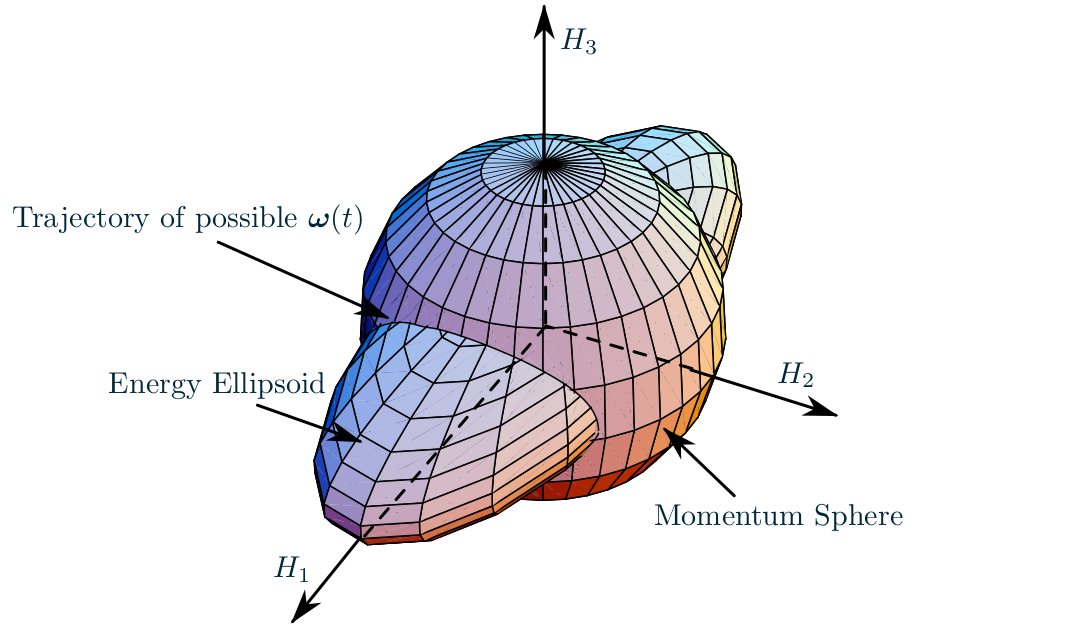
\includegraphics[width=0.7\textwidth]{Figures/momentum_energy_sphere}
	\caption{Trajectory of the polhode is at the intersection of the Momentum sphere and the Energy ellipsoid, expressed in $h$ coordinates (from \cite{schaub_spacecraft_2020})}
	\label{fig:momentum_energy_sphere}
\end{figure}

The \emph{medium-energy} case is an inflexion point between high and low energy. The intersection between the two ellipsoid is called the \emph{separatrix}. In such case, any rotation $^{B}\vect{\omega}_{B}$ will converge in one of the two intersection of the ellipsoids with the $y$ axis, in an infinite amount of time. While theoretically possible, such case never occur in practice as the energy of a real object will always be exact one required. An free-floating object whose energy level is close to medium energy will show quasi stability with $^{B}\vect{\omega}_{B}$ close to the $y$, then a sudden change to the other end. This effect is known as the \emph{Dzhanibekov} effect, or \emph{tennis-racket} theorem.


%------------------------------------------------------------------------------
%------------------------------------------------------------------------------
\section{Sensing the world}\label{C2:sensing}
\subsection{Optoelectronics sensors}

% Missions qui ont volé avec une caméra, une caméra en stéréovision et un Cameras and LiDAR
Europe has demonstrated the ability to fly autonomously for proximity operations with the \gls{atv} for automatic rendezvous and docking to the \gls{iss}. While taking advantage of GPS signals in \gls{leo} for coarse navigation, the systems switched to lasers-reflectors relative navigation 250m before docking \citep{fehse_automated_2003}. The same system has been used by DARPA's Orbital Express mission with a cooperative spacecraft \citep{howard_orbital_2008}. This mission was designed to demonstrate "short-range and long-range autonomous rendezvous, capture and berthing, on-orbit electronics upgrades, on-orbit refuelling, and autonomous fly-around visual inspection" \citep{friend_orbital_2008}. Such fly-around and inspection have also been attempted by the \emph{XSS-10} mission \citep{davis_xss-10_2004} where a small satellite has been ejected from a Delta II rocket stage and orbited around it thanks to relative navigation dynamics. Using \gls{imu} and camera navigation, it aimed at taking pictures of the stage. In Europe, the \emph{PRISMA/FFIORD} demonstrated vision-navigation between a chaser and a target with a bearing-only sensor (camera). The target had two emitting \gls{led} and chaser's camera had a filter on their wavelength \citep{delpech_results_2013}. The \emph{Space Shuttle} demonstrated the use of the so-called \emph{TriDAR} on STS-128 and STS-131. This sensor makes use and fuse data from a thermal camera and a 3D Ranging sensor. This sensor has been used for relative navigation around a known target \citep{ruel_space_2012}.

% Papiers qui présentent une approche de la navigation visuelle (caméra only)
While some equipment and experiments have already flown in the past, relative visual navigation for proximity operations remains an active area of research. Camera-only relative navigation has been also extensively studied with known or partially known uncooperative targets. Straight-Forward thinking would place a predefined known marker on the target allowing fast and accurate visual detection under several lighting conditions, therefore reconstructing relative pose between both spacecraft \citep{wen_robust_2017}. If no pre-defined markers available, one can take advantage of design constraints of a satellite (therefore restricting the problem only to objects presenting this accessory). For every heavy satellite launched, the interface between the launcher and the satellite (known as "launcher ring") present a recognisable feature across devices and can, therefore, be searched in the image to recover relative orientation (orthogonal invariant) and even pose if dimensions of the ring is known \citep{xu_pose_2012}. If shape knowledge of the spacecraft is known then relative pose can be directly extracted from the image by aligning the 3D model with the perception thanks to ICP algorithm as elegantly demonstrated in \citep{aghili_prediction_2012}. A recent review on visual-based navigation algorithms with a known target and experimental tests is available in \citep{pesce_experimental_2019}.

% Papiers qui présentne un combo cqméra LiDAR ou lIdar only.
Under the taxonomy of \gls{lidar} lies several technologies that are not all suited for space applications. Three categories arise: the scanning devices, the sensor-based on detector array and the spatial light modulator \citep{blais_review_2004, crosby_multiphase_2011, kirmani_exploiting_2011}. Scanning devices ember one detector and present some moving parts to orient a laser beam according to a specific cyclic pattern. This operation mode makes the sensor not well suited for space application as any moving mechanism present the risk of failure. In addition, the measuring time between one cyclic pattern to the next can create measuring discrepancies in case of relatively rapid motion. Scannerless detectors don't have any moving part thus alleviating the motion blur problem. The scene is illuminated and the array of sensors measure the light returning to the source. These \gls{lidar}s, however, are more challenging to calibrate and the spatial resolution is fixed by design (sensor array). In both categories, depth from laser is performed by \gls{cw} or \gls{pw} techniques. \gls{cw}-\gls{lidar} measure distances thanks to the phase-shift of a coherent signal bouncing back from the target. Due to the phase ambiguity problem, this technology is typically used for close-range applications (below 15m). \gls{pw}-\gls{lidar}s on the other hand measure time for photons of an incoherent source to bounce back from the target, hence the common name of \gls{tof} \gls{lidar}s. The range accuracy is limited by the time precision of the receiver but the operational range can go from a few meters to a few kilometres, making them ideal candidates for orbital scenarios. Finally, the spatial light modulator uses illumination patterns on the target surface and observe thanks to a camera analogue sensor the projections and compute from then shape and depth of the observation. Performances of this last category make them unsuitable for spaceflight as of now \citep{opromolla_review_2017}.

A \gls{tof}-\gls{lidar} has been incorporated in the \emph{RAVEN} mission launched in 2017 to determine the relative pose of the vehicles visiting the \gls{iss} \citep{strube_raven:_nodate}. Another sensor has been incorporated in the\emph{OSIRIS-REX} Asteroid Sample Return mission for enabling relative navigation \citep{lauretta_osiris-rex_2015}. Finally, \emph{ORION} multi-purpose crew vehicle hosts NASA's TriDAR, a \gls{tof}-\gls{lidar}, which will be the main cooperative relative navigation sensor \citep{roback_helicopter_2013}.

\subsection{Image processing}
An array of pixels representing an image usually has to undergo some algorithm to extract useful information to be used. Two paradigms are available: either \emph{dense} methods which tends to use all information available in the image, or \emph{sparse} methods that are making a first compression of the data by computing interest points in the image by the use of \emph{feature detectors} that will elect point of interest in the image. While the dense method extracts the most information out of the image by using every pixel, the computational requirements of such method makes its use unreasonable for embedded systems without dedicated hardware such as graphic cards \citep{szeliski_computer_2011}. For this reason, the remainder of this section will focus on sparse features.

%\todo{Explain feature detector and feature decriptor}
A point of interest in a given image is generally detected by a \emph{feature detector} with the main goal of detecting salient points so that, given two neighbours images, the same point should be detected in both. The detection algorithm as well as the quality measure to decide upon acceptation or rejection of the feature depends on the chosen algorithm. Once a feature is detected, a \emph{feature descriptor} is extracted from the image at the feature location as description of the feature. Given two features detected in similar images, a comparison between feature descriptor shall assess if both features represent the same point in the world or not. Several algorithm and techniques for feature detection and description are available in the literature.

A detection of good features to track is proposed in \cite{shi1994good} where the corners are detected in the image using the pixel gradients. The eigenvalues of the gradient of a patch of pixel around the detected features are used as a quality measure to keep or discard the detected corner. The \gls{sift} detector searches for local extrema in image filtered with differences of Gaussian \cite{lowe_object_1999}, also known as \emph{blob} detection. \gls{sift} has been considered for a long time as state of the art, leading to \gls{surf} aiming at improving the computation and robustness of \gls{sift}. To enhance performances, a faster detection based on a the Hessian matrix approximation was proposed \citep{leonardis_surf:_2006}. An open-source alternative has been proposed in 2001 with the \gls{orb} descriptor, based on \gls{fast} keypoint detector \citep{leonardis_machine_2006}. The latter extracts feature key points faster than difference of Gaussian or Hessian matrix approximation. \gls{orb} also propose the enhancement of the \gls{brief} visual descriptor \cite{hutchison_brief:_2010}, by allowing to store its orientation. \gls{orb} aims at providing a faster alternative to \gls{sift} \cite{rublee_orb:_2011}. It has been demonstrated in textured environment that \gls{orb} is equally or more accurate than  its \gls{sift} and \gls{surf} counterparts with a fraction of the computation time \cite{karami_image_2017}. Another feature descriptor has been proposed with \gls{freak} where the detection of features is inspired by the biological retina. This descriptor claims better performances, faster with lower memory usage than detectors cited above \cite{alahi_freak:_2012}. 

A complete paradigm shift from detector/descriptors has been proposed in \cite{detone_toward_2017} where two chained \gls{cnn} takes two images as an input, computes salient points in the two images with the first network and outputs an estimated homography between the two frames. The correlation between salient points can then be performed using the estimated homography and choosing the closest neighbours.

Matching features between images, i.e comparing all descriptors and retaining the one with the highest similarities is a way to track features in frames. In the case of two consecutive images resulting from a smooth motion of the camera, however, a solution relying on the \emph{optical-flow} is possible with the \gls{lk} tracking algorithm \cite{bourget_pyramidal_1999}. The optical flow corresponds to the pattern of apparent motion os the scene between several consecutive frames, caused by the motion of the object or the camera. The tracker assumes that neighbouring pixels exhibit the similar motion and that pixel intensities stays similar between the two frames. With such assumptions, the \gls{lk} tracker takes 3*3 pixel patch around the feature and tries to find the displacement that minimises the pixel error.

This work uses the gradient-based feature detection algorithm presented in \cite{shi1994good} for detecting new features in a given image, and tracking features frame-to-frame is performed using the described \gls{lk} algorithm. The main motivation herein lies with the development at Airbus Defence and Space of the Themis software for orbital and planetary vision-based navigation \cite{djafari-rouhani_genevis_2019}. Their implementation features a space-certified feature detector and \gls{klt} tracker, an enhanced version of the aforementioned \gls{lk} tracker \cite{tomasi1992shape} which has been successfully tested on a LEON4 space-qualified computer.

\subsection{Sensors models}
Different elements require a modelling of the \gls{oe} sensors, from the simulation needs to the inner working of the proposed algorithm. The camera and depth sensors can be modelled in various ways, depending on the actual hardware and use-case \cite{szeliski_computer_2011, hartley_multiple_2003}. 

\begin{figure}
    \centering
    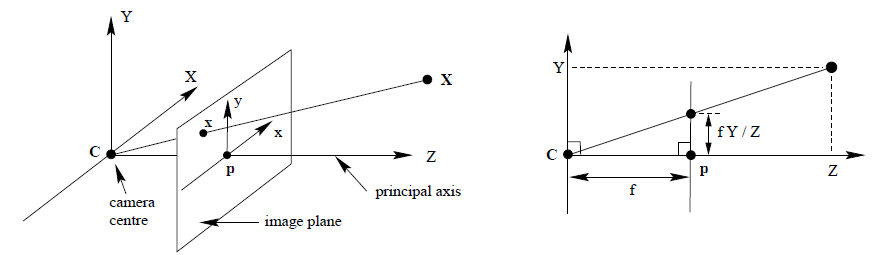
\includegraphics[width=\textwidth]{Figures/camera_pinhole_model}
    \caption{Camera pinhole model (from \cite{hartley_multiple_2003})}
    \label{fig:camera_model}
\end{figure}

The camera is modelled using the \emph{pinhole} camera model. This model assume that the distance between the point and the camera is much bigger that the focal length $f$, and is representative of most cameras that are not subject to high distortions. Given a 3D point $^{C}\vect{p} = \left[x, \: y, \: z \right]^{\intercal}$ in the camera frame, the projection in the \emph{image plane} is given by:
\begin{equation}
		\eqnmark[black]{image}{\begin{bmatrix}
		u \\ v \\ 1	
		\end{bmatrix}} = \mat{K} \: 
		\eqnmark[black]{normalised}{\begin{bmatrix}
			\sfrac{x}{z} \\ \sfrac{y}{z} \\ 1
		\end{bmatrix}}
\end{equation}
\annotate{below, left}{image}{image coordinates}
\annotate{below, right}{normalised}{normalised image plane coordinates}
%\vspace{0.5em}

The coordinates $(u, \:v)$ are the \emph{image coordinates} expressing the position of the projection of the point $^{C}\vect{p}$ on the sensor, in meters. The \emph{intrinsics} matrix $\mat{K}$ defines the inner parameters of the camera and projects the \emph{normalised} image coordinates to the \emph{image coordinates}. This matrix is defined as:
\begin{equation}
	\mat{K} = \begin{bmatrix}
              f & s  & c_x\\ 
              0 & af & c_y\\ 
              0 & 0  & 1 
           \end{bmatrix} 
\end{equation}
where $f$ is the \emph{focal length}, the parameters $c$ are the coordinates of the optical centre ($c = (0,0)$ means that the origin of film coordinates is at the centre of the sensor), $a$ is the \emph{aspect ratio} for  different focal length on $x$ and $y$, and $s$ is the \emph{skew} that encode the possible non perpendicularity of the sensor with the optical axis. Usually $a = 1$ and $s = 0$. This camera intrinsics is generally known as either communicated by the manufacturer of is recovered using the chessboard calibration algorithm \cite{szeliski_computer_2011}.
The \emph{normalised image coordinates} is an abstraction from the specific parameters of a given camera and corresponds to a pinhole camera model of a focal length $f = 1m$. The projection from the image coordinates to the normalised ones can be transformed using $\mat{K}^{-1}$. Such abstraction is useful when working with the pinhole camera model without making any assumption about the camera parameters. In this work the \emph{normalised image coordinates} are used unless specified otherwise. When using images from a specific camera, the keypoints detected in the image expressed in image coordinates are transformed back into the normalised image coordinates using the known camera intrinsics.

As outlined above, depth sensing can be achieved by very different hardware, with all their specific models. In the present work, no assumption about a specific sensor is being made. The model therefore becomes the simple L2-norm of the considered point in the sensor frame $\{ C \}$:
\begin{equation}
	d = \left \| {}^{C}\vect{p} \right \|
\end{equation}


\section{Filtering}\label{C2:filters}

\subsection{Kalman Kilter}
Kalman filter is a Bayes filter for linear models proposed in the 60s, providing the estimate mean $\hat{\boldsymbol{x}}_t$ and covariance $\hat{\text{P}}_t$ of an unknown true state $\boldsymbol{x}_t$ at the time $t$, given noisy measurements $\boldsymbol{z}$. Under the assumption of unbiased Gaussian noise, the Kalman filter is an optimal estimator. It can be decomposed in two main steps: an \emph{update} and a \emph{correction} step. Given a state vector $\hat{\boldsymbol{x}}$ and its associated covariance matrix $\text{P}$, the update part of the filter propagates state and its covariance from time $t-\Delta t$ to time $t$ using the linear state-space transition matrix $\text{F}$:
\begin{align}
    \hat{\boldsymbol{x}}^{+}_t &= \text{F}(\Delta t) \: \boldsymbol{x}_{t-\Delta t} \label{eq:kalman_linear_update}\\
    \hat{\text{P}}^{+}_t &= \text{F}(\Delta t) \: \hat{\text{P}}_{k-\Delta t} \: \text{F}(\Delta t)^\intercal + \hat{\text{V}}(\Delta t) \label{eq:kalman_linear_update_covariance}
\end{align}
with the process noise covariance matrix $\hat{\text{V}}$. To distinguish the intermediary results of the \emph{update} part with the following step, it is here noted with the subscript $(\cdot)^{+}$. Once measurements $\boldsymbol{z}_{t}$ are available, expected measurements are computed from the estimated state $ \hat{\boldsymbol{x}}^{+}_t $ with the linear state-space measurement model $\text{H}$. The difference is referred to as the \emph{innovation} $\boldsymbol{\nu}$:
\begin{equation} \label{eq:kalman_linear_innovation}
    \boldsymbol{\nu} = \boldsymbol{z}_{t} - \text{H}\hat{\boldsymbol{x}}^{+}_t
\end{equation}
The Kalman gain $\text{K}$ is computed using propagated state covariance, sensor model and its associated noise covariance matrix $\hat{\text{W}}$ to reflect the amount of correction to apply on the state vector given the innovation and the state covariance.
\begin{equation} \label{eq:kalman_linear_gain}
    \text{K} = \hat{\text{P}}^{+}_t \text{H}^\intercal \left( \text{H}\hat{\text{P}}^{+}_t \text{H}^\intercal + \hat{\text{W}} \right)^{-1}
\end{equation}
Finally, state and covariance can be corrected:
\begin{align}
    \hat{\boldsymbol{x}}_t&= \hat{\boldsymbol{x}}^{+}_t + \text{K}\boldsymbol{\nu}  \label{eq:kalman_linear_correct} \\
    \hat{\text{P}}_t &= \hat{\text{P}}^{+}_t - \text{K}\text{H}\hat{\text{P}}^{+}_t  \label{eq:kalman_linear_correct_covariance}
\end{align}

\subsection{Extended Kalman Filter}

However, most models are not linear, thus calling for the need of an extension of the previously outlined algorithm. The \gls{EKF} offers to apply Kalman filtering to non-linear motion $\boldsymbol{f}(\cdot)$ and/or observation models $\boldsymbol{h}(\cdot)$ by using a first-order approximation of models for covariance propagation. While this allows the use of the Kalman filter formulation with a non-linear model, it breaks the underlying Gaussian assumption of the linear filter, rendering the estimator non-optimal. Despite this apparent limitation, it has been practically found very successful in various domains \cite{corke_robotics_2017}. State vector update and innovation are therefore computed with:
\begin{align}
    \hat{\boldsymbol{x}}^{+}_t &= \boldsymbol{f}( \boldsymbol{x}_{t-\Delta t}, \Delta t) \label{eq:ekf_update} \\
    \boldsymbol{\nu} &= \boldsymbol{z}_{t} - \boldsymbol{h}(\hat{\boldsymbol{x}}^{+}_t) \label{eq:ekf_innovation}
\end{align}
and covariance update and correction are kept as replacing in \cref{eq:kalman_linear_update, eq:kalman_linear_update_covariance} and \cref{eq:kalman_linear_gain, eq:kalman_linear_correct_covariance}, replacing $\text{F}$ and $\text{H}$ with the Jacobians of $\boldsymbol{f}(\cdot)$ and $\boldsymbol{h}(\cdot)$ respectively:
\begin{align}
    \text{F}_t &= \frac{ \partial\boldsymbol{f}(\hat{\boldsymbol{x}}^{+}_t) }{ \partial\hat{\boldsymbol{x}}^{+}_t } \\
    \text{H}_t &= \frac{ \partial\boldsymbol{h}(\hat{\boldsymbol{x}}^{+}_t) }{ \partial\hat{\boldsymbol{x}}^{+}_t }
\end{align}

\subsection{Error-State Kalman Filter}
The former two filters estimate the state vector $\hat{\boldsymbol{x}}$ in linear and non-linear cases. \gls{ESKF} breaks down the state vector into two parts: a nominal state $\bar{\boldsymbol{x}}_t$, predicted by the dynamic model $\boldsymbol{f}(\cdot)$ and an error state $\delta\boldsymbol{x}_t$, compensating errors induced by noise and integration. \gls{ESKF} offers to integrate nominal state outside the filtering scheme:
\begin{equation}
    \bar{\boldsymbol{x}}_t = \boldsymbol{f}( \boldsymbol{x}_{t-\Delta t}, \Delta t) \label{eq:eskf_update_nominal} \\
\end{equation}
and estimate the error $\delta\boldsymbol{x}_t$ and its covariance between predicted nominal state $\bar{\boldsymbol{x}}_t$ and true state $\boldsymbol{x}_t$ given measurements $\boldsymbol{z}$ and linear (or linearised) dynamical and sensor model at the nominal state:
\begin{align}
    \hat{\text{P}}^{+}_{(\delta \boldsymbol{x}, t)} &= \text{F}(\Delta t) \: \hat{\text{P}}_{k-\Delta t} \: \text{F}(\Delta t)^\intercal + \hat{\text{V}}(\Delta t) \\
    \hat{\delta \boldsymbol{x}}_t &= \text{K}\boldsymbol{\nu} \\
    \hat{\text{P}}_{(\delta \boldsymbol{x}, t)} &= \hat{\text{P}}^{+}_t - \text{K}\text{H}\hat{\text{P}}^{+}_t
\end{align}
with:
\begin{align}
\text{F}_t &= \frac{ \partial\boldsymbol{f}(\hat{\boldsymbol{x}}^{+}_t) }{ \partial\delta\hat{\boldsymbol{x}}^{+}_t } \\
\text{H}_t &= \frac{ \partial\boldsymbol{h}(\hat{\boldsymbol{x}}^{+}_t) }{ \partial\delta\hat{\boldsymbol{x}}^{+}_t }
\end{align}

Estimated error can then be injected into the nominal state with a suitable composition:
\begin{align}
\hat{\boldsymbol{x}}_t &= \bar{\boldsymbol{x}}_t \otimes \delta\hat{\boldsymbol{x}_t} \label{eq:eskf_correct_state} \\
\delta\hat{\boldsymbol{x}}_{t+\Delta t} &= 0
\end{align}
and covariance of the error updated to reflect this correction.

%------------------------------------------------------------------------------
%------------------------------------------------------------------------------
\section{Gaussian Processes}\label{C2:gaussian_processes}
\subsection{Regression}
% Qu'est-ce qu'une GP regression et en quoi c'est différent d'une regression classique 
Given a dataset of observed data $\vect{y}$ at given points $\vect{X} = \left [\vect{x}_1, \: \cdots \: , \vect{x}_n \right ]$, $\vect{x}_i \in \mathbb{R}^{m}$, we would like to infer the value of $y_\ast$ at the new point $\vect{x}_\ast$. A usual approach to this problem is the simple regression problem where a chosen function $\hat{\vect{y}} = f(\vect{\theta}, \vect{x})$ is fitted to the data, that is the functions parameters $\vect{\theta}$ are tuned to minimise error between the expectation and the training data $e=\hat{y} - y$ with the hope that these parameters will generalise. This \emph{model-based} regression is heavily dependant of the function $f$ chosen by the designer. An acute knowledge of the underlying process is necessary to allow a meaningful regression and inference. 

Gaussian Processes is a machine-learning tool solving the regression problem using another approach, by describing the distribution over the possible functions given the dataset. Once the \gls{gps} are trained over the given dataset, the most likely function is drawn from the distribution and evaluated at the requested $\vect{x}_\ast$. A \gls{gp} model is described by its mean function $\mu(\vect{x})$ and its covariance function $k(\vect{x}, \vect{x}')$, and written as \cite{murphy_machine_2012}:
\begin{equation}
	f(\vect{x}) \sim \text{GP}(\mu(\vect{x}), k(\vect{x}, \vect{x}'))
\end{equation}
with the mean and covariance function defined as:
\begin{align}
\mu(\vect{x}) &=\mathbb{E}[f(\vect{x})] \\
k\left(\vect{x}, \vect{x}^{\prime}\right) &=\mathbb{E}\left[(f(\vect{x})-m(\vect{x}))\left(f\left(\vect{x}^{\prime}\right)-m\left(\vect{x}^{\prime}\right)\right)\right]
\end{align}

One can already see the very nice property of \gls{gps} with the above definition : when inferring on a datapoint $\vect{x}_\ast$, the \gls{gp} returns the most likely value at the requested point with the mean function, but also the estimated variance thanks to the covariance function. 
\begin{figure}
	\centering
	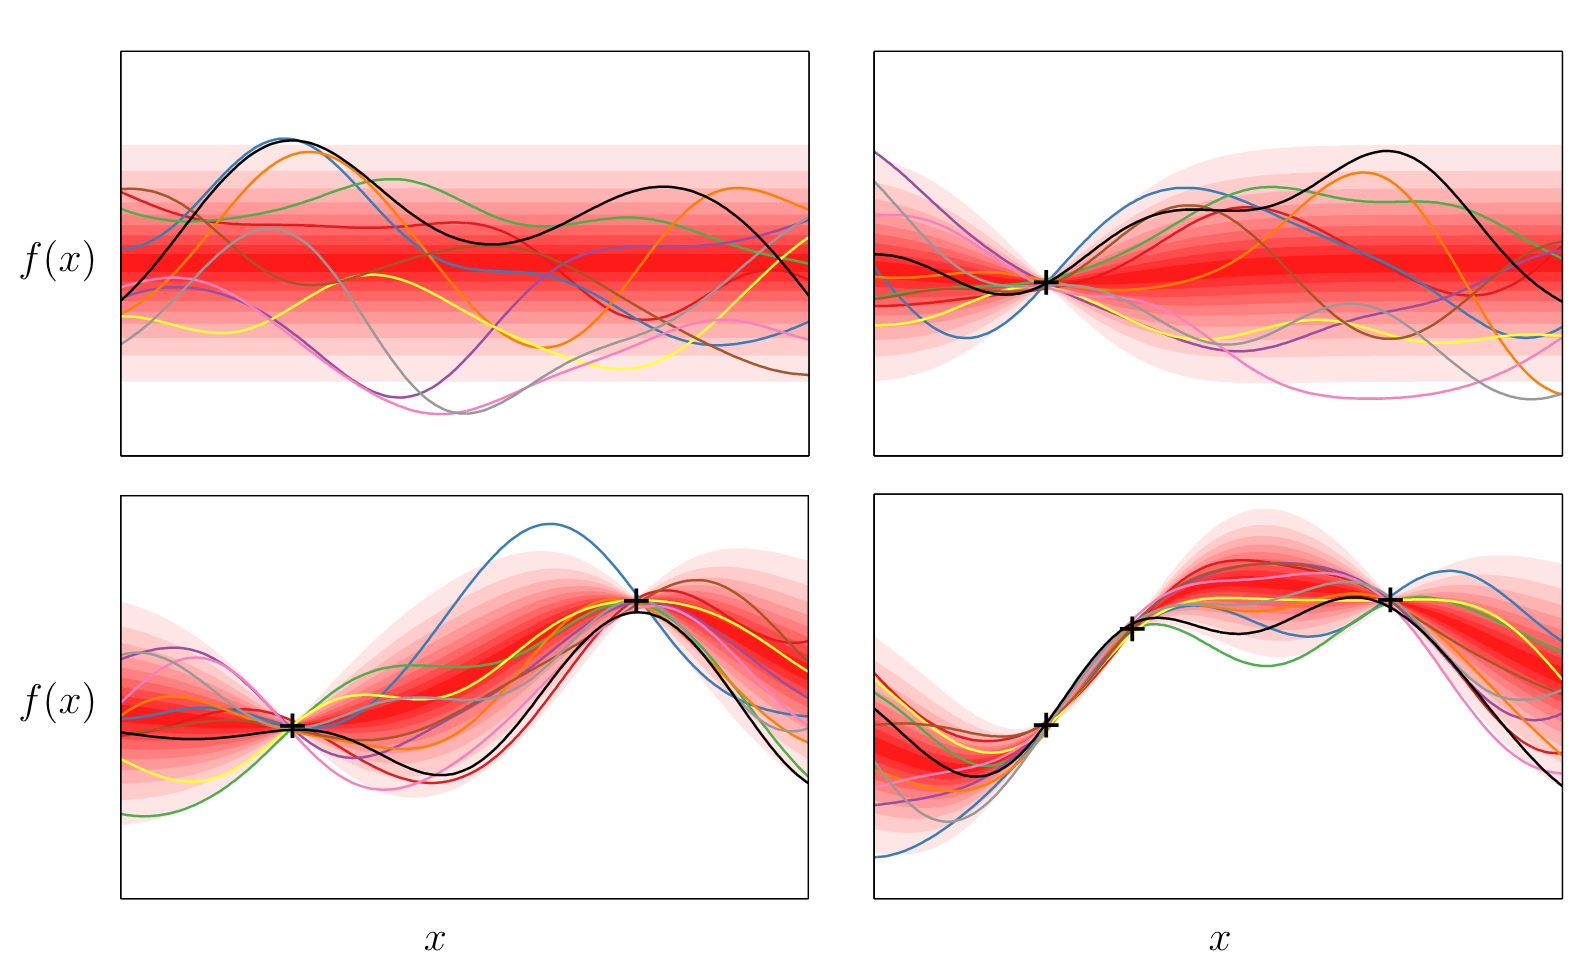
\includegraphics[width=\textwidth]{Figures/gp_draw.png}
	\caption{Example of a GP predictions. The shades indicate the percentiles of the predicted density while the coloured lines are the sampled functions from the process. At the beginning, no data is available and the functions are centred in zero. As data comes in, the possible functions pass by the training points and the covariance shrinks at these points. (from \cite{duvenaud_automatic_2014})}
	\label{fig:gp_draw}
\end{figure}

The prediction of the \gls{gp} is possible thanks to the \emph{conditioning} of the joint Gaussian distribution to the observations. If we note $\vect{f}(\vect{X}) = \left[f(\vect{x}_1, \cdots, \vect{x}_n  \right]$, then the inference at a point $\vect{x}_\ast$ is given by:
\begin{equation}\label{eq:gp_prediction}
\begin{aligned}
p\left(f\left(\vect{x}_\ast\right) \mid \vect{f}(\vect{X}) \cdot \vect{X}, \mu, k\right)=\mathcal{N}(&f\left(\vect{x}_{\ast}\right) \mid \mu\left(\vect{x}_\ast \right)+k\left(\vect{x}_{\ast}, \vect{X}\right) k(\vect{X} \cdot \vect{X})^{-1}(\vect{f}(\vect{X})-\mu(\vect{X})), \\
&k\left(\vect{x}_{\ast}, \vect{x}_{\ast}\right)-k\left(\vect{x}_{\ast}, \vect{X}\right) k(\vect{X}, \vect{X})^{-1} k\left(\vect{X}, \vect{x}_{\ast}\right))
\end{aligned}
\end{equation}

The covariance function $k$ is computed between each element of $\vect{X}$ to construct the covariance matrix which will then be used to make the inference at the requested test points. This function express how the different points of $\vect{X}$ relate to each other, and is chosen by the designer depending on the knowledge of the data structure to which \gls{gps} are applied. Different covariance function encompass different behaviour, detailed in next subsection. They all share the presence of one or several \emph{hyper-parameters} $\vect{\theta}$ allowing fitting to the training-set characteristics. Therefore, the training step of \gls{gps} consist of \emph{tuning} the kernel's hyper-parameters $\theta$ for best fitting the training data. This is performed by maximising the marginal likelihood of the \gls{gp} distribution based on the observed data.

While often difficult to compute, the marginal likelihood of a \gls{gp} is given by \cite{duvenaud_automatic_2014}:
\begin{equation} \label{eq:gp_marginal_likelihood}
\begin{aligned}
p(\vect{f}(\vect{X}) \mid \vect{X}, \mu, k) &=\mathcal{N}(\vect{f}(\vect{X}) \mid \mu(\vect{X}), k(\vect{X}, \vect{X})) \\
&=(2 \pi)^{-\frac{1}{2}} \times |k(\vect{X}, \vect{X})|^{-\frac{1}{2}} \\
&\times \exp \left\{-\frac{1}{2}(\vect{f}(\vect{X})-\vect{\mu}(\vect{X}))^{\intercal} k(\vect{X}, \vect{X})^{-1}(\vect{f}(\vect{X})-\vect{\mu}(\vect{X}))\right\}
\end{aligned}
\end{equation}

Therefore, the training process consist into finding the parameters $\theta$ maximising the \cref{eq:gp_marginal_likelihood}. In practice, such operation is performed by minimising the negative log marginal likelihood using a \emph{gradient descent} based approach, like the ADAM solver \cite{murphy_machine_2012}.
\begin{equation}
\begin{aligned}
\vect{\theta}_{opt} &=\underset{\vect{\theta}}{\operatorname{argmax}}(p(\vect{f}(\vect{X}) \mid \vect{X}, \mu, k)) \\
&= \underset{\vect{\theta}}{\operatorname{argmin}}(-\log(p(\vect{f}(\vect{X}) \mid \vect{X}, \mu, k)))
\end{aligned}
\end{equation}

% Quels sont les avantages et les inconvénients des GPs
The advantages of \gls{gps} is twofold. First, as outlined above, a \gls{gp} prediction over a test point data provides the expected value but also the estimated covariance given the training set. This property allows a very nice integration of \gls{gps} in a Bayesian filtering scheme as proposed in \cite{ko_gp-bayesfilters_2008}. Secondly, the presence of a handful parameters $\vect{\theta}$ for tuning the algorithm, compared to other machine learning techniques, makes the fit over the hyper-parameters easier and, more importantly, easily interpretable for a human. The main drawback of \gls{gps} is the computational load in $\mathcal{O}(N^3)$ as both training and the inference in \cref{eq:gp_marginal_likelihood, eq:gp_prediction} require the computation of the inverse of the covariance matrix. In practice $\vect{X}$ must be chosen in accordance to the hardware capacity.

\subsection{Covariance function}
% Montrer l'impact de la covariance function sur l'apprentissage de la structure
Given all the training points $\vect{X}$, the covariance function $k$, also called \emph{kernel}, is used to compute the covariance matrix linking all the points together and, ultimately, allowing the prediction of the mean and covariance at a new test point $\vect{x}_\ast$. Therefore, the covariance function \emph{encodes} the expected behaviour of the modelled process and conditions the prediction given the test training set. This function is key design parameter un the application of \gls{gps} to the dataset and knowledge of the underlying behaviour is beneficial for choosing the right function. A representation example of different kernels is presented on \cref{fig:gp_kernels_examples}.

% Quels kernels existent dans la nature
\begin{figure}
     \centering
     \begin{subfigure}[b]{0.3\textwidth}
         \centering
         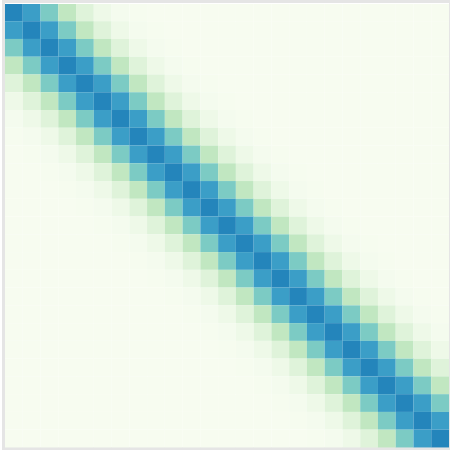
\includegraphics[width=\textwidth]{Figures/kernel_rbf.png}
         \caption{RBF Kernel}
         \label{fig:kernel_rbf}
     \end{subfigure}
     \hfill
     \begin{subfigure}[b]{0.3\textwidth}
         \centering
         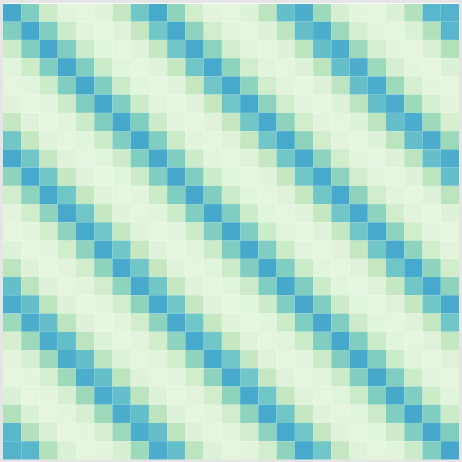
\includegraphics[width=\textwidth]{Figures/kernel_periodic.png}
         \caption{Periodic}
         \label{fig:kernel_periodic}
     \end{subfigure}
     \hfill
     \begin{subfigure}[b]{0.3\textwidth}
         \centering
         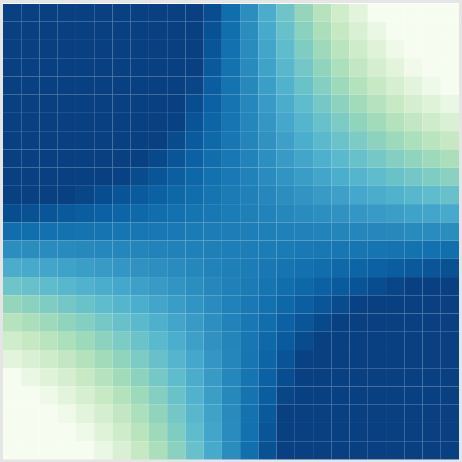
\includegraphics[width=\textwidth]{Figures/kernel_linear.png}
         \caption{Linear}
         \label{fig:kernel_linear}
     \end{subfigure}
        \caption{Three different kernels used in Gaussian processes for equally spaced $x$. \ref{fig:kernel_rbf} shows the relation of a data point is with its direct neighbours and weakens as the data points are further away. \ref{fig:kernel_periodic} is adapted for the periodic dataset where the relationship between two points is periodic. \ref{fig:kernel_linear} puts a lot of correlation between points at the extremity of the dataset and where the function i expected to  change side in the middle. (from \cite{gortler_visual_2019})}
        \label{fig:gp_kernels_examples}
\end{figure}

The main four kernels are the following:
\begin{itemize}
	\item The \emph{Radial basis function} kernel, or \emph{squared exponentional} encodes the local variations of the function: close points $x$ and $x'$ have their values $f(x)$ and $f(x')$ correlated as they are close. As the distance grows, they start to loose influence over each other to finally become unrelated. The kernel is formulated as:
		\begin{equation}
		k(x, x') = \sigma^{2}\exp\left(- \frac{(x - x')^{2}}{2l^2} \right)
		\end{equation} where the hyper-parameter $\sigma^2$, the variance, encodes the average distance from the function's mean and $l$, the \emph{length-scale}, represents the length of the influence region between data points. This kernel is often used as a default kernel when no knowledge of the underlying process is at hand. Predictions on $x_\ast$ are close to the data points and go towards 0 as the test point is away from the training set.
	\item The \emph{periodic}, or \emph{exp-sin-squared} kernel is particularly suited for periodic signals as its name suggest. The \cref{fig:kernel_periodic} clearly shows the recurrent weights added to the different points spaced of the defined period. The prediction at $x'$ is highly correlated to the training points $\vect{x}$ spaced on the modulo of the period. This kernel is defined as:
		\begin{equation}
		k(x, x') = \sigma^{2}\exp\left(-\frac{2}{l^2} \sin^2 \left( \frac{\pi(x-x')}{p}\right) \right )
		\end{equation} where the parameters $\sigma$ and $l$ have the same meaning of above. The parameter $p$ encodes the periodicity.
	\item The \emph{linear} kernel are encoding a linear trend in the data. The sampled functions with this kernel are straight lines crossing the x-axis at a certain location with uncertainty. The mathematical expression is:
		\begin{equation}
			k(x, x') = \sigma^{2}(x-c)(x'-c)
		\end{equation} with $c$ the intersection point of all the functions, and $\sigma^2$ as above.
	\item The \emph{white noise} kernel is generally used to integrate the sampling noise of the dataset, preventing the sampled functions to pass exactly at the training points but integrate also some noise. The kernel is simply:
		\begin{equation}
			k(x, x') =  \left\{\begin{matrix}
        n & x = x'\\ 
        0 & x \neq x'
        \end{matrix}\right.
		\end{equation} with $n$ the noise level.
\end{itemize}

Other kernels are available for Gaussian Processes, encompassing different data structure and finding other uses and interested reader can find more information in \cite{murphy_machine_2012}. Kernels can be added and multiplied together to represent a more complex data structure as a combination of the basic structure each represent. The addition between kernels represent an element-wise addition of each kernel values. As such, it can be though as an \emph{AND} operation. For example, the addition of a linear with a periodic kernel would encompass a signal with a general trend and a locally repeating structure. In contrary, the multiplication of kernels can be thought as a "OR" combination as they both have to be high so the signal can pass. A multiplication between a linear and a periodic kernel will encompass a repeating data structure whose amplitude increase or decrease as the distance between $x$ and $x'$ grows.

In this work, we use the \gls{gps} implementation offered by Scikit-Learn, a Python library specialised in Machine-Learning \cite{scikit-learn}. Despite other implementations available, the use of this library is motivated by its ground in the field and the availability and versatility of its \gls{api}.

\section{Discussion and Summary}


\clearpage

\lhead{\textit{Chapter3}}
\chapter[Chapter Title]{\label{cha:Chapter3}Chapter Title}

%------------------------------------------------------------------------------
%------------------------------------------------------------------------------
\section{\label{C3:Section1}Section 1}

%------------------------------------------------------------------------------
\subsection{\label{C3:SubSection11}Subsection 1.1}

%------------------------------------------------------------------------------
\subsection{\label{C3:SubSection12}Subsection 1.2}

%------------------------------------------------------------------------------
%------------------------------------------------------------------------------
\section{\label{C3:Section2}Section 2}




\clearpage

\lhead{\textit{Chapter4}}
\chapter[Chapter Title]{\label{cha:Chapter4}Chapter Title}

%------------------------------------------------------------------------------
%------------------------------------------------------------------------------
\section{\label{C4:Section1}Section 1}

%------------------------------------------------------------------------------
\subsection{\label{C4:SubSection11}Subsection 1.1}

%------------------------------------------------------------------------------
\subsection{\label{C4:SubSection12}Subsection 1.2}

%------------------------------------------------------------------------------
%------------------------------------------------------------------------------
\section{\label{C4:Section2}Section 2}
\clearpage

%\lhead{\textit{Chapter5}}
%\chapter[Chapter Title]{\label{cha:Chapter5}Chapter Title}

%------------------------------------------------------------------------------
%------------------------------------------------------------------------------
\section{\label{C5:Section1}Section 1}

%------------------------------------------------------------------------------
\subsection{\label{C5:SubSection11}Subsection 1.1}

%------------------------------------------------------------------------------
\subsection{\label{C5:SubSection12}Subsection 1.2}

%------------------------------------------------------------------------------
%------------------------------------------------------------------------------
\section{\label{C5:Section2}Section 2}
%\clearpage

%\lhead{\textit{Chapter6}}
%\chapter[Chapter Title]{\label{cha:Chapter6}Chapter Title}

%------------------------------------------------------------------------------
%------------------------------------------------------------------------------
\section{\label{C6:Section1}Section 1}

%------------------------------------------------------------------------------
\subsection{\label{C6:SubSection11}Subsection 1.1}

%------------------------------------------------------------------------------
\subsection{\label{C6:SubSection12}Subsection 1.2}

%------------------------------------------------------------------------------
%------------------------------------------------------------------------------
\section{\label{C6:Section2}Section 2}
%\clearpage
%
%\lhead{\textit{Chapter7}}
%\chapter[Chapter Title]{\label{cha:Chapter7}Chapter Title}

%------------------------------------------------------------------------------
%------------------------------------------------------------------------------
\section{\label{C7:Section1}Section 1}

%------------------------------------------------------------------------------
\subsection{\label{C7:SubSection11}Subsection 1.1}

%------------------------------------------------------------------------------
\subsection{\label{C7:SubSection12}Subsection 1.2}

%------------------------------------------------------------------------------
%------------------------------------------------------------------------------
\section{\label{C7:Section2}Section 2}
%\clearpage

\lhead{\textit{Conclusions}}
\chapter[Chapter Title]{\label{cha:Chapter8}Conclusions}

%------------------------------------------------------------------------------
%------------------------------------------------------------------------------
\section{\label{C8:Section1}Conclusions}

%------------------------------------------------------------------------------
%------------------------------------------------------------------------------
\section{\label{C8:Section2}Limitations and Future Work}





\clearpage

%% ----------------------------------------------------------------
% References and Appendices
\lhead{\textit{Appendices}}
%------------------------------------------------------------------------------
\appendix
%----------------------------------------------------------------------------
%----------------------------------------------------------------------------
\chapter{\label{app:Appendix}Appendix}
\clearpage

\begin{spacing}{1.3}
\renewcommand\bibname{References}
\lhead{\textit{References}}
\cleardoublepage
\phantomsection % Again required for correct page numbering
\addcontentsline{toc}{chapter}{References}
\bibliography{References/library}
\end{spacing}

\end{document}
%% ----------------------------------------------------------------